\documentclass[12pt]{article}
\usepackage{setspace}
\usepackage{subfigure}
\usepackage{geometry}
\geometry{left=1in,right=0.75in,top=1in,bottom=1in}
\usepackage{placeins}
\usepackage{float}
\usepackage{soul}
\usepackage{mathtools}
\usepackage{framed}
\usepackage{listings}

\renewcommand{\vec}{\mathbf}

\usepackage{amsmath,amssymb,amsthm}
\usepackage[colorlinks = true,
    linkcolor=blue,
    filecolor=magenta,      
    urlcolor=cyan]{hyperref}

\usepackage{graphicx} % Required for inserting images

\onehalfspacing

\title{Summer Datathon 2024 \\ \large Team 7}
\author{Arjun Ashok\footnote{equal contribution} \and Ekeoma Osondu \and Pramana Saldin* \and Grace Wang*}
\date{August 2024}

\begin{document}

\maketitle

\section{Guiding Question}
\textbf{Do periods with low meat production track with overall unemployment numbers?}

\section{Executive Summary}
We concluded that there is a \textbf{negative correlation} between meat production and unemployment present in the dataset, i.e., \textbf{lower meat production leads to higher unemployment}.

Using \textbf{lag analysis}, we were able to conclude that \textbf{the strength of the correlation between meat production and unemployment rates is between 0.1 and 0.2}. In both of the methods we chose (cross-correlation and mutual information regression), the optimal lag was positive, which indicates that \textbf{it is likely that changes in unemployment rates follow changes in meat production amounts}.

Using this correlation, we were able to use meat production data as a factor in determining unemployment, and we used an $\mathrm{ARIMA}(1,1,0)$ model to predict future unemployment rates \textbf{with some confidence}. 

% In this report, we examine whether periods of low meat production correlate with overall unemployment numbers. We start by noting the significance of the meat industry to the economy, employing more than 30 percent of food and beverage workers in the United States \cite{31_Percent}. Among the provided datasets, our primary focus was on using meat production figures from Livestock $\&$ Meat Domestic Data and unemployment numbers from the American Community Survey. Our analysis involved conducting correlation analyses and ARIMA models for predicting and forecasting. 
In future research, we aim to employ Long Short-Term Memory models, decision-trees, and neural-based architecture to develop more robust predictive models and to get a better gauge of feature importance.

\section{Background}
Meat production is a significant sector in the economy, providing countless employment opportunities across all stages of the process, from farming to processing and distribution. Meat consumption has fluctuated in the United States in the past few decades, but it has been steadily increasing in recent years. In particular, from 1999 to 2006, meat consumption averaged over 250 pounds per capita. Then, it fell from 2007 to 2013 following the Great Recession, and then increased every year from 2015 to 2019 \cite{Illinois}. With fluctuating demand for meat, there has also been change in employment opportunities for workers within both the meat production industry and related industries, such as feed production and equipment manufacturing. 

As estimated by the U.S. Department of Agriculture, meat and poultry plants employed nearly 31 percent of food and beverage manufacturing workers in the U.S. in 2021 \cite{31_Percent}. From the U.S. Census Bureau, it appears that workers in the meat industry are disproportionately immigrants or from rural parts of the United States. The meatpacking industry is concentrated in the Midwest and Plains states, whereas the poultry industry is concentrated in the Deep South \cite{Economic_Policy_Institute}.

How, then, do fluctuations in meat production correlate with unemployment? How might changes in unemployment affect the meat production industry? There are many different arguments around this topic. For instance, Scott Brown from the University of Missouri actually argues that low unemployment might hinder meat production capacity because competition for jobs makes it more difficult to add shifts and thus increase the efficiency of meat production \cite{Brownfield}. The answers to these questions could predict what might happen in a hypothetical transition to cultivated and plant-based meats. Morais-da-Silva, Villar, Reis et al. have noted that experts from different countries have shown different views toward the expected impact of plant-based meats. According to their research, Brazilian professionals believe that cultivated meat has the potential to create new and higher-skilled jobs, while experts from Europe were more skeptical of these conclusions \cite{Plant_Based}.

In this work, we will examine the correlation between meat production and overall unemployment numbers. We will be making use of public data from Livestock $\&$ Meat Domestic Data and American Community Survey to answer these questions.

\section{Methods}
    \subsection{Dataset Engineering}
        \subsubsection{Cleaning}
        While the data was pre-cleaned to an extent, it remained far from being directly deployable in its initial state. As such, we opted to further pre-process the data to not only ensure we kept the most relevant information, i.e. ignoring features that provided little utility in answering our guiding question, but also filtered out suspicious/outlier/NaN data points.
        
        For instance, in the dataset from the American Community Survey, only the unemployment data provided utility. So, we filtered out information that was less pertinent to our guiding question, such as health insurance coverage or commute to work. In particular, we only left the unemployment rates (also referred to as percent unemployed in the data) and percent errors.

        There were also null data points in some of the datasets. For example, in the cold storage dataset, there was no data for the amount of broiler chicken stored before 2003. As a result, we had to filter out these data points to ensure the accuracy of the dataset.

        \subsubsection{Transformation}
        One of the key issues across the datasets was a temporal misalignment, i.e. we had data for timelines that didn't fully overlap. Given the lack of open-source synthetic time series generation, \footnote{e.g. T-SMOTE, the state-of-the-art technique by Microsoft Research for upsampling time-series, remains closed source despite its high projected efficacy}\cite{T_SMOTE}, we opted instead to truncate the timelines across the board to the most restricting dataset. Specifically, the unemployment rates provided in the economic characteristics dataset only spanned from 2010 $\to$ 2022 inclusive. Luckily, this was the most restrictive the timeline would get, and therefore we could truncate all other data sources to roughly match this timeline $\pm6 - 12$ months.

        In the process of cleaning the meat datasets, we also opted to consolidate certain data points based on the type of meat. Instead of distinguishing between beef, veal, pork, or lamb and mutton, we aggregated all corresponding values with the same month and year into a single data point categorized as red meat. Similarly, data points for broiler, turkey, and frozen eggs with the same month and year were summed up into one data point labeled as poultry. This approach allowed us to perform a more comprehensive analysis while maintaining the ability to differentiate between potential variations in types of meat.

        For the economic characteristics data, we were given the unemployment rates broken down by state. Although we considered potentially taking a weighted average of the unemployment rates by state based on the distribution of meat industry workers, i.e. weighing the meat industry states higher, we chose to keep the sample as representative as possible of the entire working population. To accomplish this, we leveraged state population data from the U.S. Census Bureau to take a population-weighted average by state, i.e. constructing a representative mean unemployment rate for the entire United States and Territories. The graphs, correlation analysis, and time-series modeling all rely on this aggregation.

        These transformations to the datasets were made for downstream modeling and analysis. For visualizations, on the other hand, we kept the data largely intact for the sake of being able to see trends across a longer period (four decades as opposed to one decade). To make the graphs more readable, we also consolidated data points based on year for the meat production and meat storage graphs.

        \subsubsection{Imputation \& Inference}
        \begin{figure}
            \begin{minipage}{.5\textwidth}
                \centering
                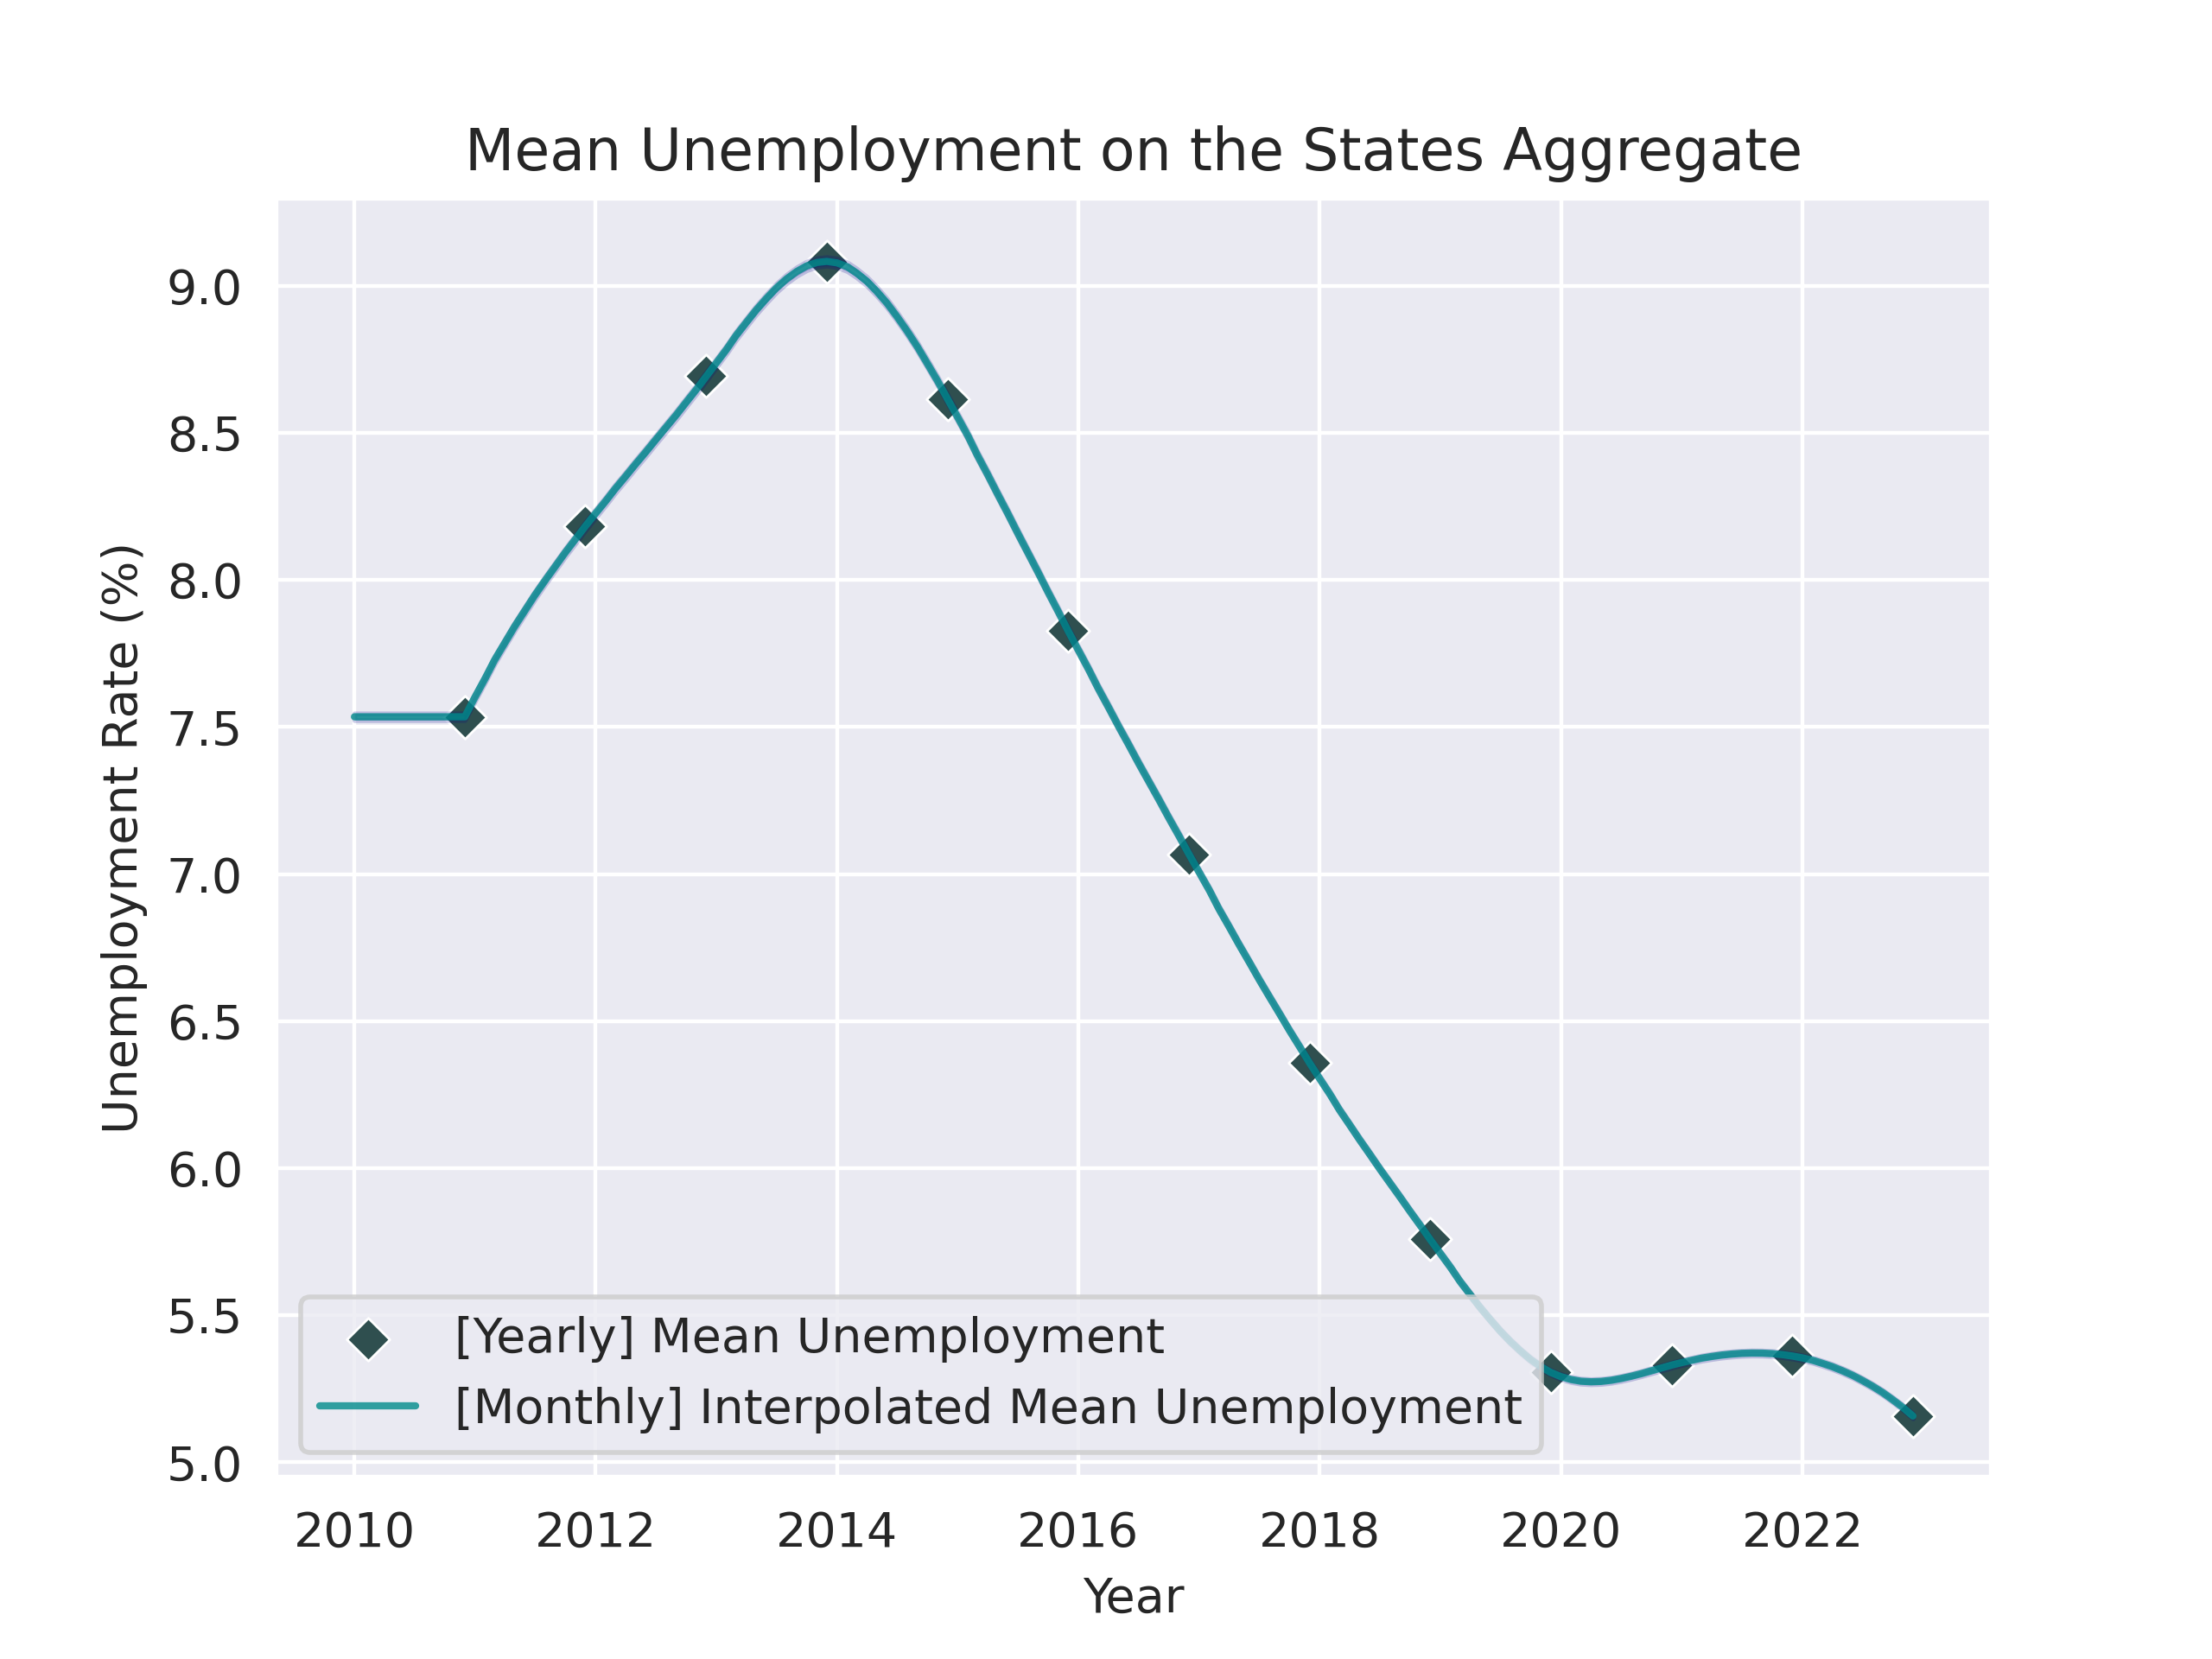
\includegraphics[width=1\linewidth]{images/Unemployment Rates - Constant.png}
                \caption{Interpolated mean unemployment data with missing 2010 data.}
                \label{fig:1_monthly_unemployment_plateau}
            \end{minipage}
            \begin{minipage}{.5\textwidth}
                \centering
                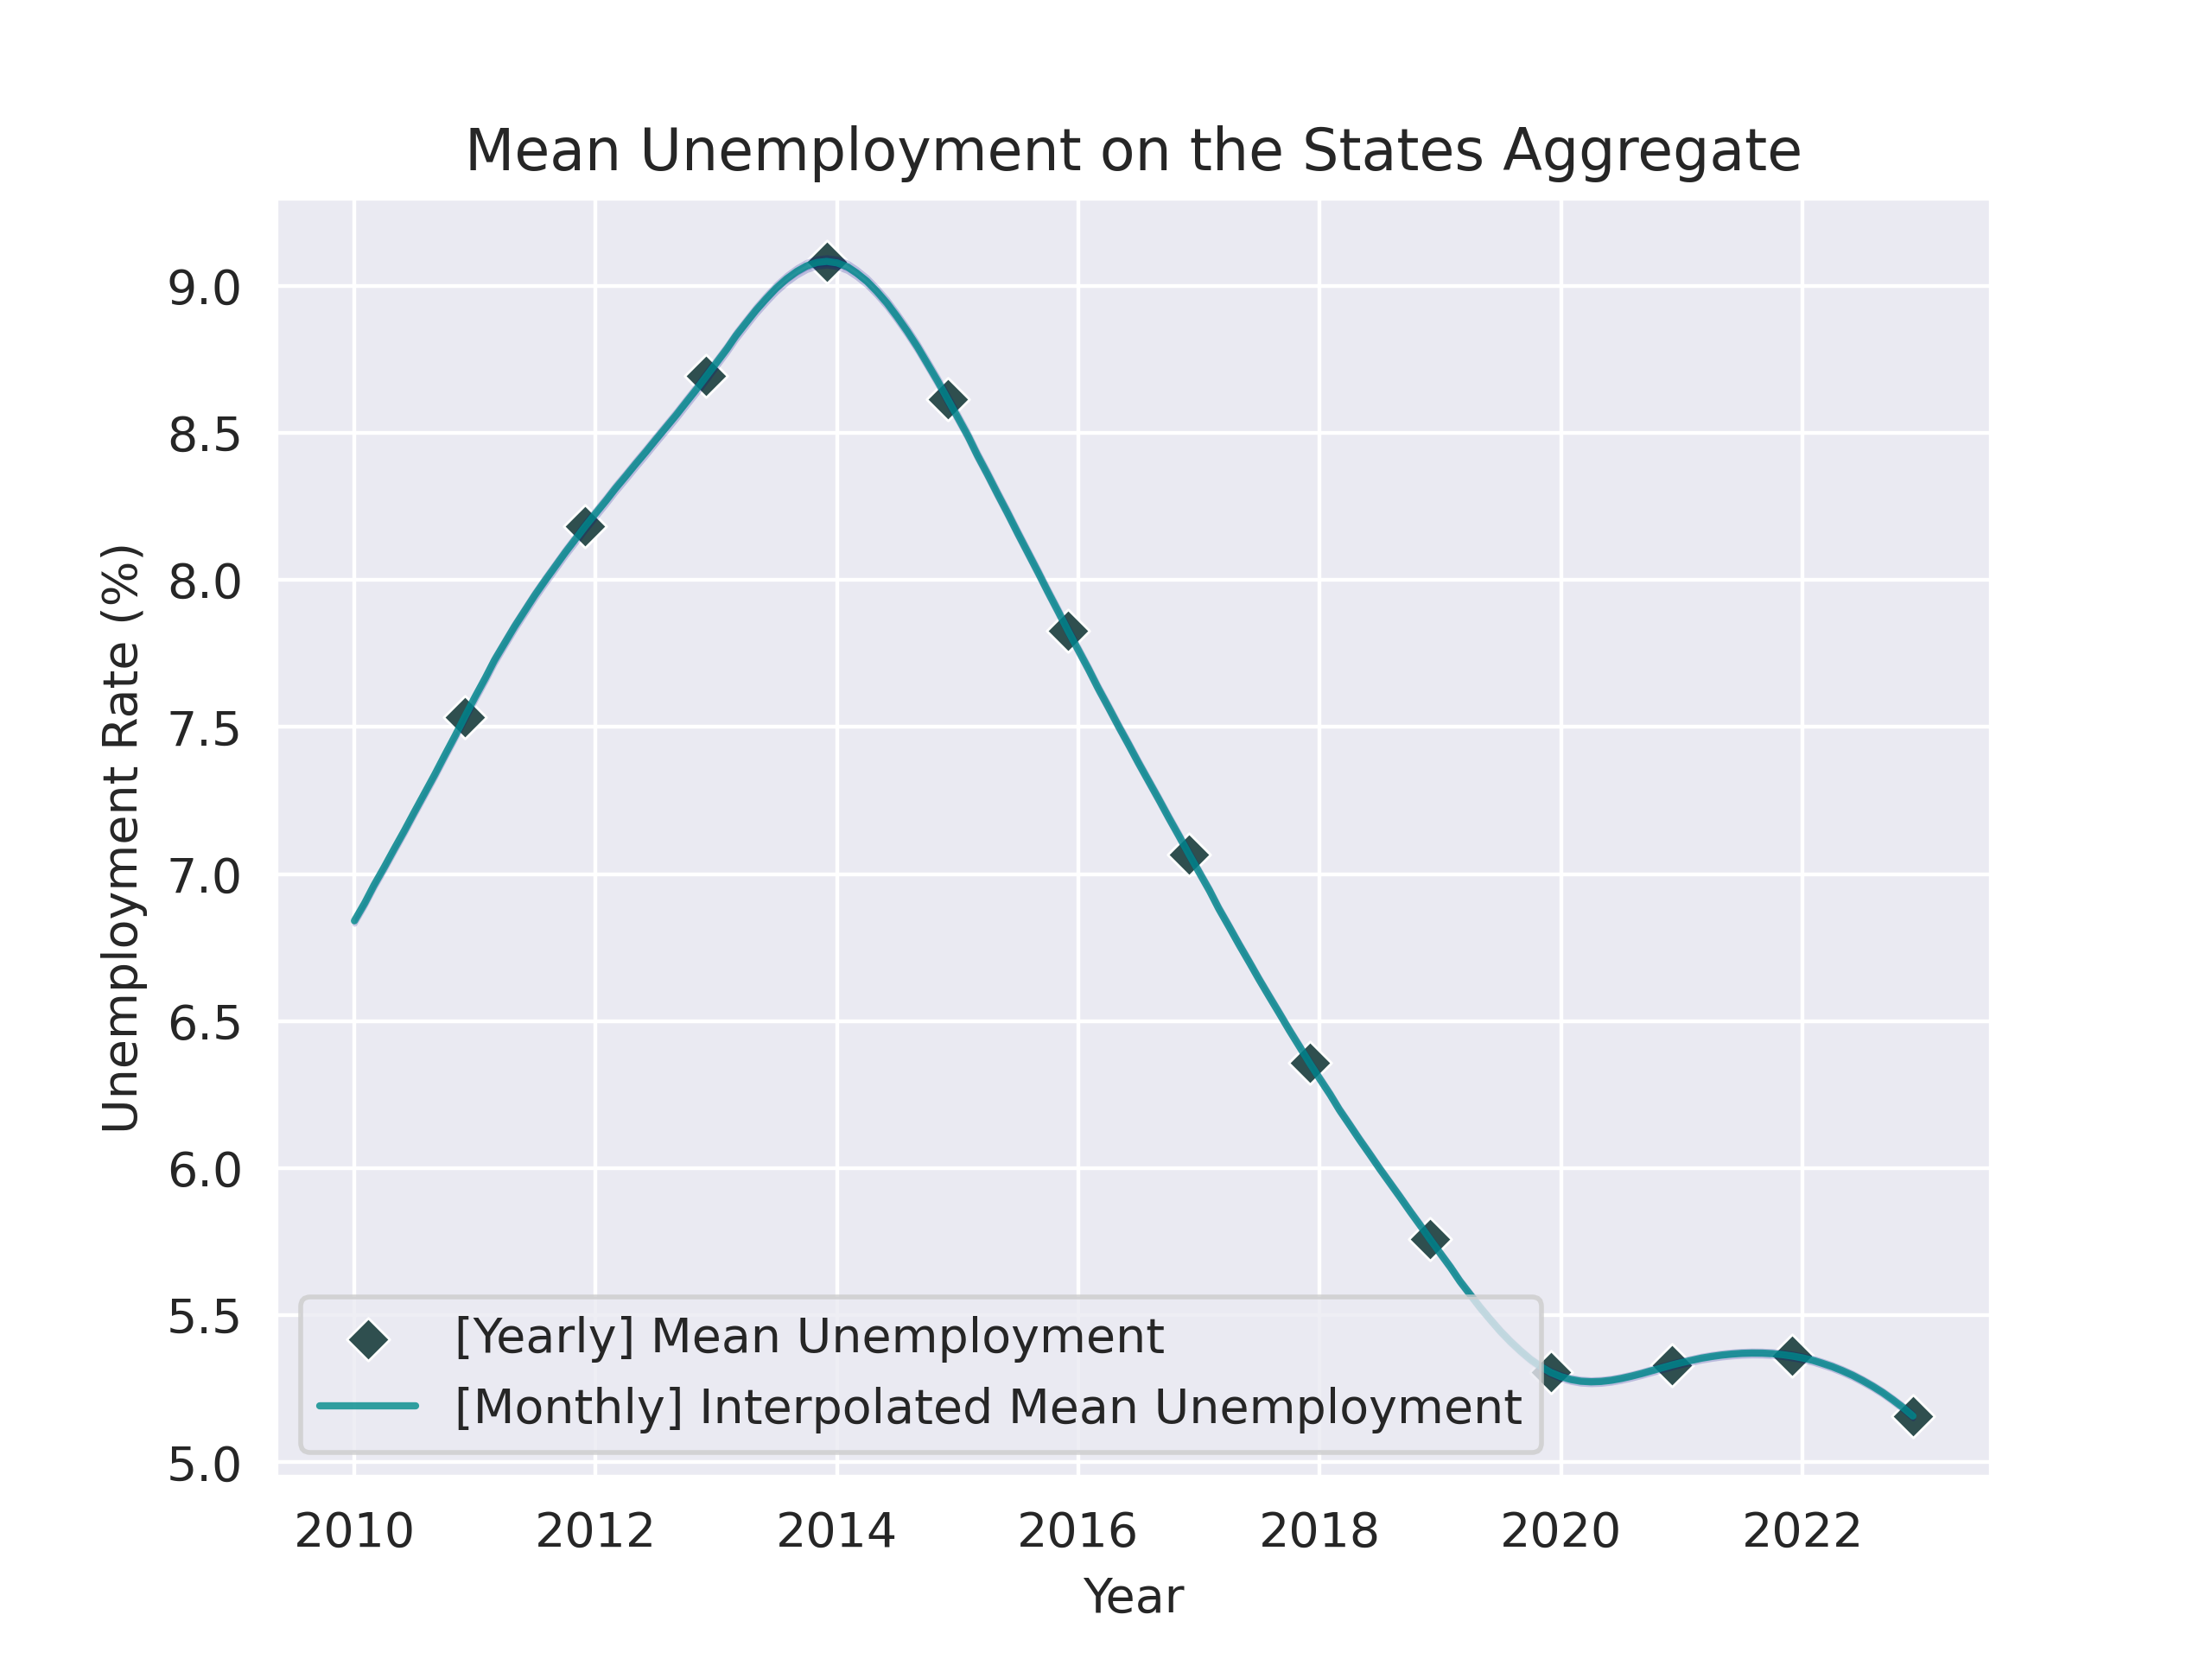
\includegraphics[width=1\linewidth]{images/Unemployment Rates.png}
                \caption{Interpolated mean unemployment data using $\mathrm{ARIMA}(1,1,0)$.}
                \label{fig:2_monthly_unemployment}
            \end{minipage}
        \end{figure}
        
        Another key challenge was the disparate temporal step sizes across datasets. Namely, the unemployment data only tracked year-over-year rates while the meat production/storage datasets tracked more granular month-by-month records. Rather than discard this granularity (which proved useful in later modeling and lag analysis), we chose to interpolate the unemployment time series instead to produce a month-by-month record, thus preserving temporal scales.
        
        To execute this, we leverage interpolation via cubic spline functions to interpolate between the yearly anchor points in the data. However, since we treat the yearly points as occurring in the last month of the year (December 1st) due to its reflective nature on the whole year, we were left with 11 data points in the months preceding the first yearly entry without anchor points to interpolate with. In other words, the first 11 months of every state's unemployment record in 2010 were missing entries; given its temporal position, this now also became an extrapolative context rather than interpolative. To remedy this, we initially chose to back-fill the entries via the earliest unemployment record we had, resulting in a plateau-like curve for the first 12 months of data \ref{fig:1_monthly_unemployment_plateau}. Given this was likely an inaccurate representation of the monthly evolution of unemployment rates, we were motivated to consider how to extrapolate backward as a means of imputation. Eventually, empirical testing showed the use of Auto-regressive Integrated Moving Average (ARIMA) models with an order of (1, 1, 0) to forecast backward trends proved robust, matching what one would expect from such a curve. The final curve smoothly interpolated between the yearly anchor points and correctly extrapolated for the months before the first entry, thus indicating a strong imputation fit \ref{fig:2_monthly_unemployment}.

    \subsection{Feature Selection}
    Given the scope of the question and the numerous datasets provided, it was essential in the early stages to constrict ourselves to only the most important datasets. This meant a thorough dive into what features could provide us utility in answering the guiding question.

    \begin{enumerate}
        \item Economics Characteristics: the economic characteristics dataset provides us with essential information about unemployment rates. Although more granular information about unemployment rates broken down by demographic factors would have proven useful in determining a representative meat industry employment rate, ultimately, we utilized the simple aggregation by state and year data to conduct our analyses.

        \item Commodities*: initially, we surmised that the commodities data could provide an interesting view into how the meat prices related to production rates, thus giving another angle into how unemployment rates are affected. Ultimately, we decided against this choice during deeper analysis.

        \item Meat Production: we leveraged this to provide the majority of our analysis on the production of meat

        \item Slaughter Counts: this dataset holds a rate-like relationship with meat production, thus proving useful in modeling since it can be directly involved with predicting unemployment among the workers in the industry

        \item Meat Storage: is likely proportional to unemployment since the more meat stored, the more likely consumption has reduced and therefore less need for workers in the industry. Less consumption can also point to less people spending which indicates recession/unemployment
    \end{enumerate}

    \subsection{Correlation Analysis}

    The primary objective of the correlation analysis was to explore and understand how variations in Meat Production might be related to changes in Unemployment rates. This involved investigating whether higher or lower meat production had any observable impact on unemployment or if the two variables are independent of each other. Generally, we found that higher meat production led to a statistically significant decrease in unemployment rates when state numbers are aggregated.
    
    \subsection{Lag Correlation Analysis}
    Predicting demand for goods has long been a driving goal for many corporations, especially those in industries reliant on manufactured goods. The chaotic nature of time series, especially on an aggregate, long-term scale, means it is also a never-ending pursuit. However, predictive modeling techniques have improved drastically in the last few decades, and thus the ability for such companies to accurately gauge future demand for products has similarly seen great strides. This observation motivated us to consider how the pre-emptive actions that companies take with regards to production rates may directly influence unemployment rates in the future. More explicitly, a company that expects demand for goods to go down either due to a recession or other motivating factors will likely act on this expectation by adjusting its production in the short term.

    The effects of this may be delayed but still present in the unemployment rates following such pre-emptive action. Thus, to test this hypothesis, we design a study in which we observe the (non-linear) cross-correlation of unemployment rates with the meat industry's production, storage, and slaughter rates when offset by a range of months. We consider this as an analogous `autocorrelation' score between features. The higher the lag correlation is for a given offset (lag), the more related those features are at those intervals. Rather than rely on one measure, we simultaneously leveraged an orthogonal metric in the form of mutual information regression (MIR) to observe how well one feature can predict the other at varying lag points, thus indicating how strongly related the two are.

    We can begin by examining the relationship between meat production and unemployment rates where one time series is shifted (lagged) by a certain number of months. In this way, we can determine whether changes in one series are related to changes in the other series after a certain delay.

    To do this, we need to first make sure both datasets (for meat production and unemployment) are aligned and cleaned, which we have described in Section 4.1.2. Because both positive and negative lags are possible, we chose to test out all possible lags from $-96$ to 96 inclusive, i.e. eight years. After calculating the cross-correlation function, we can plot all of these data points to visualize the impact that lag has on the coefficient of correlation between meat production and unemployment rates.


    \subsection{ARIMAX Predicting \& Forecasting}
    \subsubsection{ARIMA Models}
    \textbf{ARIMA} is an auto-regressive integrated moving-average model for predicting and forecasting time series data \cite{HyndmanAthanasopoulos2021}. Suppose we have a set of data points $\vec{y} = (y_1,y_2,\dots)$ in a time series. We can take the difference between consecutive terms (possibly multiple times) to get a difference sequence $\vec{y}' = (y_1',y_2',\dots)$.
    An ARIMA model takes three parameters, $p$, $d$, and $q$, and takes the form:

    \begin{equation}
        \mathrm{ARIMA}(p,d,q)\colon \qquad y_t' = c + \underbrace{\phi_1 y_{t-1}' + \cdots \phi_p y_{t-p}'}_{(1)} + \underbrace{\theta_1 \varepsilon_{t-1} + \cdots + \theta_q\varepsilon_{t-q}}_{(2)} + \varepsilon_t.
    \end{equation}
    (1) represents the autoregressive part of the model, which uses lagged values of $y_{t-i}'$ to predict the current value $y_t'$, and (2) represents the moving average part of the model, which uses past errors in the forecast to predict the future $y_t'$ value. The parameter $d$ indicates how many times to take the difference sequence of $\vec{y}$. We also assume that $\varepsilon_t \sim \mathcal{N}(0, \sigma^2)$. The ARIMA model will use the data to learn the parameters $\phi_1,\dots,\phi_p$ and $\theta_1,\dots,\theta_q$.
    
    In a survey of methods for predicting unemployment by Davidescu et. al. they mention previous models using $\mathrm{ARIMA}(1,1,0)$ models have performed well in simulating unemployment in Canada \cite{Davidescu2021ComparativeAO}.
    This model is given by 
    \begin{equation}
        \mathrm{ARIMA}(1,1,0)\colon \qquad y_t' = c + \phi_1 y_{t-1}' + \varepsilon_t.
    \end{equation}
    Notice that having $d=1$ implicitly assumes that the first difference of the data is stationary (i.e. the mean and variance do not change significantly over time).

    We could have also analyzed using an ARMA model, however, given that ARMA is primarily designed for data that is stationary by itself.

    \subsubsection{Incorporating Exogenous Variables}
    A variable $X$ (concerning another variable $Y$) is said to be \textbf{exogenous} if $X$ causes or influences $Y$, but $Y$ does not cause or influence $X$ \cite{box2015time}. Our correlation analysis indicated that meat production \textit{did} influence unemployment numbers, so we therefore treated meat production data as an exogenous variable to the unemployment rate. 

    \textbf{ARIMAX} is a modification of ARIMA that accounts for exogenous variables. The form of, e.g. $\mathrm{ARIMAX}(1,1,0)$, is the following: 
    \begin{equation}
        y_t' = c \beta X + \phi_1 y_{t-1}' + \varepsilon_t.
    \end{equation}

    \subsubsection{Predicting vs. Forecasting}
    There are two different ways we can evaluate the data. Firstly, we can pass in the existing data $y_{t-1}'$ into the model and see where it predicts the next data point will be. This technique, where we use in-sample data, is called \textbf{predicting}. On the other hand, if we reach the end of the data, we could use previously predicted values as data points for ARIMA. This method of using out-of-sample data is called \textbf{forecasting}. As expected, forecasting will come with growing error, so we will have larger confidence intervals as we go out further. We will analyze both of these methods in our results. 

    % An exogenous variable is defined as a variable that is independent of the variable we are currently analyzing. 
% correlation analysis
% moving average analysis
% time series analysis
% machine learning ?
% plotting and visualizations

\section{Results \& Discussion}

We can begin by visualizing the data to discern the trends in meat production and storage over the past decades. This will be achieved by plotting amounts of meat production and storage over time. In the plot below in \ref{fig:meat_production} of production of meat over time, we can see that red meat production has experienced significant increase over the past century, albeit with some fluctuations, especially notable around the 1940s to 1950s. Poultry production, on the other hand, started from a much lower base and has seen steady and continuous increase since then. It seems like the production of red meat still dominates meat production in terms of weight, although poultry production has seen a more consistent increase.

\begin{figure}[H]
    \centering
    \begin{minipage}{.5\textwidth}
        \centering
        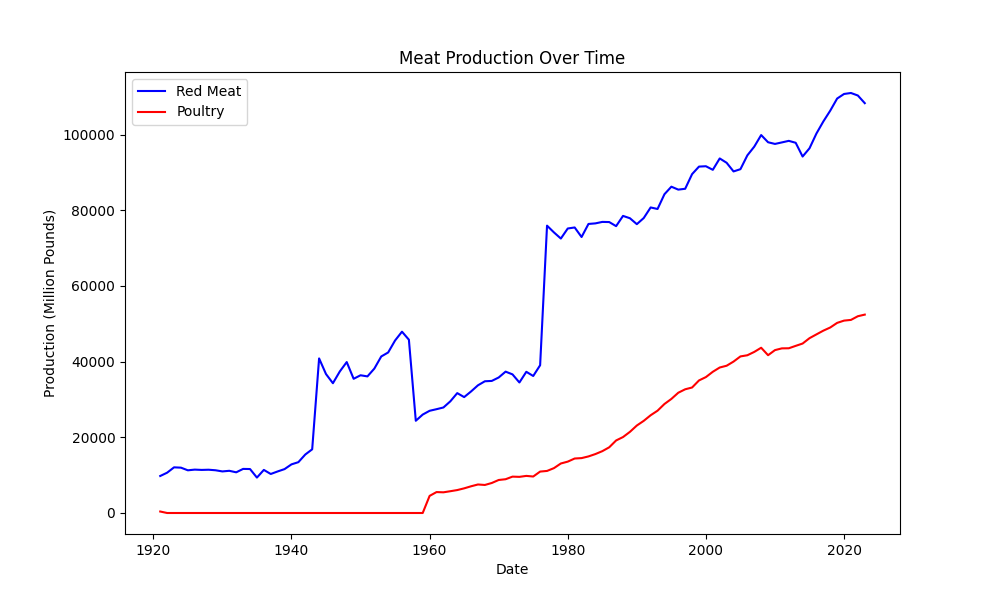
\includegraphics[width=1\linewidth]{images/Meat Production.png}
        \caption{Production of Meat Over Time}
        \label{fig:meat_production}
    \end{minipage}
\end{figure}

We can see trends in the specific species of animal being in cold storage in \ref{fig:meat_storage}. The figure on the left hand side shows that the storage of broiler meat remains relatively high compared to the storage of turkey and frozen eggs (note that there is no data on storage of broiler meat before 2003). The figure in the middle shows that beef and pork dominate the cold storage quantities for red meat, reflecting increased production and consumption trends for these types of meat. On the other hand, less common types of meat, such as veal or lamb, maintain a stable but minimal presence in cold storage. Finally, the figure on the right shows that poultry has overtaken red meat as the primary type of meat in cold storage (in terms of weight).

\begin{figure}[H]
    \centering
    \subfigure{
        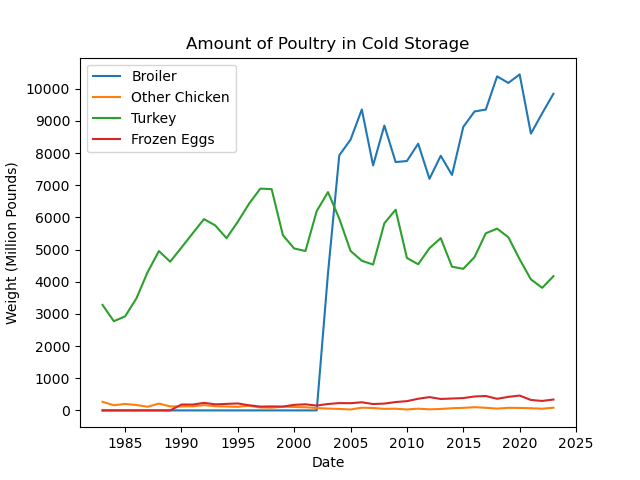
\includegraphics[width=0.3\textwidth]{images/Poultry Cold Storage.png}
    }
    \subfigure{
        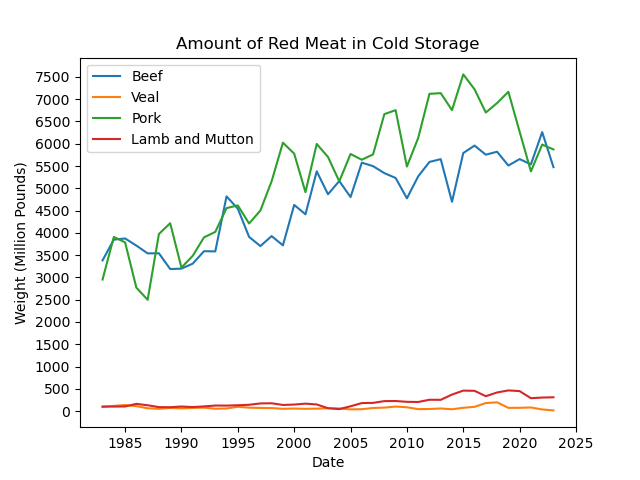
\includegraphics[width=0.3\textwidth]{images/Red Meat Cold Storage.png}
    }
    \subfigure{
        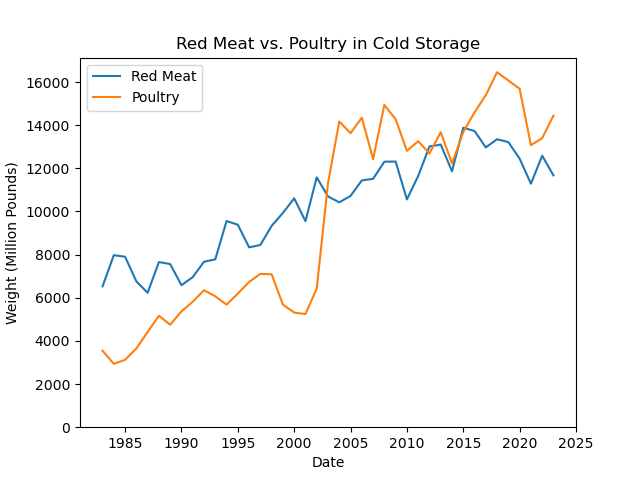
\includegraphics[width=0.3\textwidth]{images/Red Meat vs. Poultry Cold Storage.png}
    }
    \caption{Cold Storage of Meat Over Time}
    \label{fig:meat_storage}
\end{figure}

The plot below in \ref{fig:lag} shows the results of lag analysis using the metric of the cross-correlation function. It seems like the cross-correlation function between meat production and unemployment rates are consistently close to $-0.1$ across various lags, between $\pm 8$ years, which is surprisingly uniform. The plot also highlights that the lag that results in the largest absolute correlation is at 10 months. If this is accurate, it suggests that changes in meat production might happen before changes in unemployment; i.e. a possible explanation is that if meat producers anticipate a recession, then they might reduce meat production in response to reduced demand. Also, it appears that in the graph there is a cycle every five months or so, especially for positive lag. The figure in \ref{fig:lag} also shows that the coefficient of correlation is consistently negative, which matches what we expected. Intuitively, one would expect that lower meat production correlates with higher unemployment and vice versa.

The figure in \ref{fig:lag_mir}, however, shows a different story. This is the plot that we generated by using mutual information regression on the two time series. It suggests that the maximum correlation occurs when the lag is at 73 months, and the plot indicates that the strength of the maximum correlation is around 0.20 (notice that the graph includes correlation strengths).

\begin{figure}[H]
    \centering
    \begin{minipage}{.5\textwidth}
        \centering
        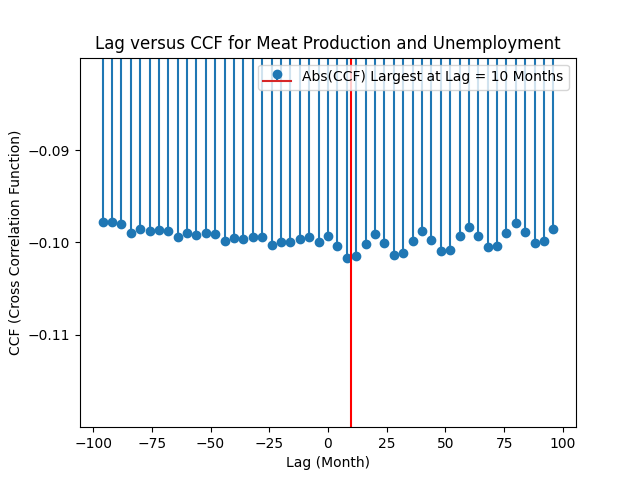
\includegraphics[width=1\linewidth]{images/Lag Correlation Coefficients.png}
        \caption{Lag Versus Cross-Correlation Function}
        \label{fig:lag}
    \end{minipage}
    \begin{minipage}{.5\textwidth}
        \centering
        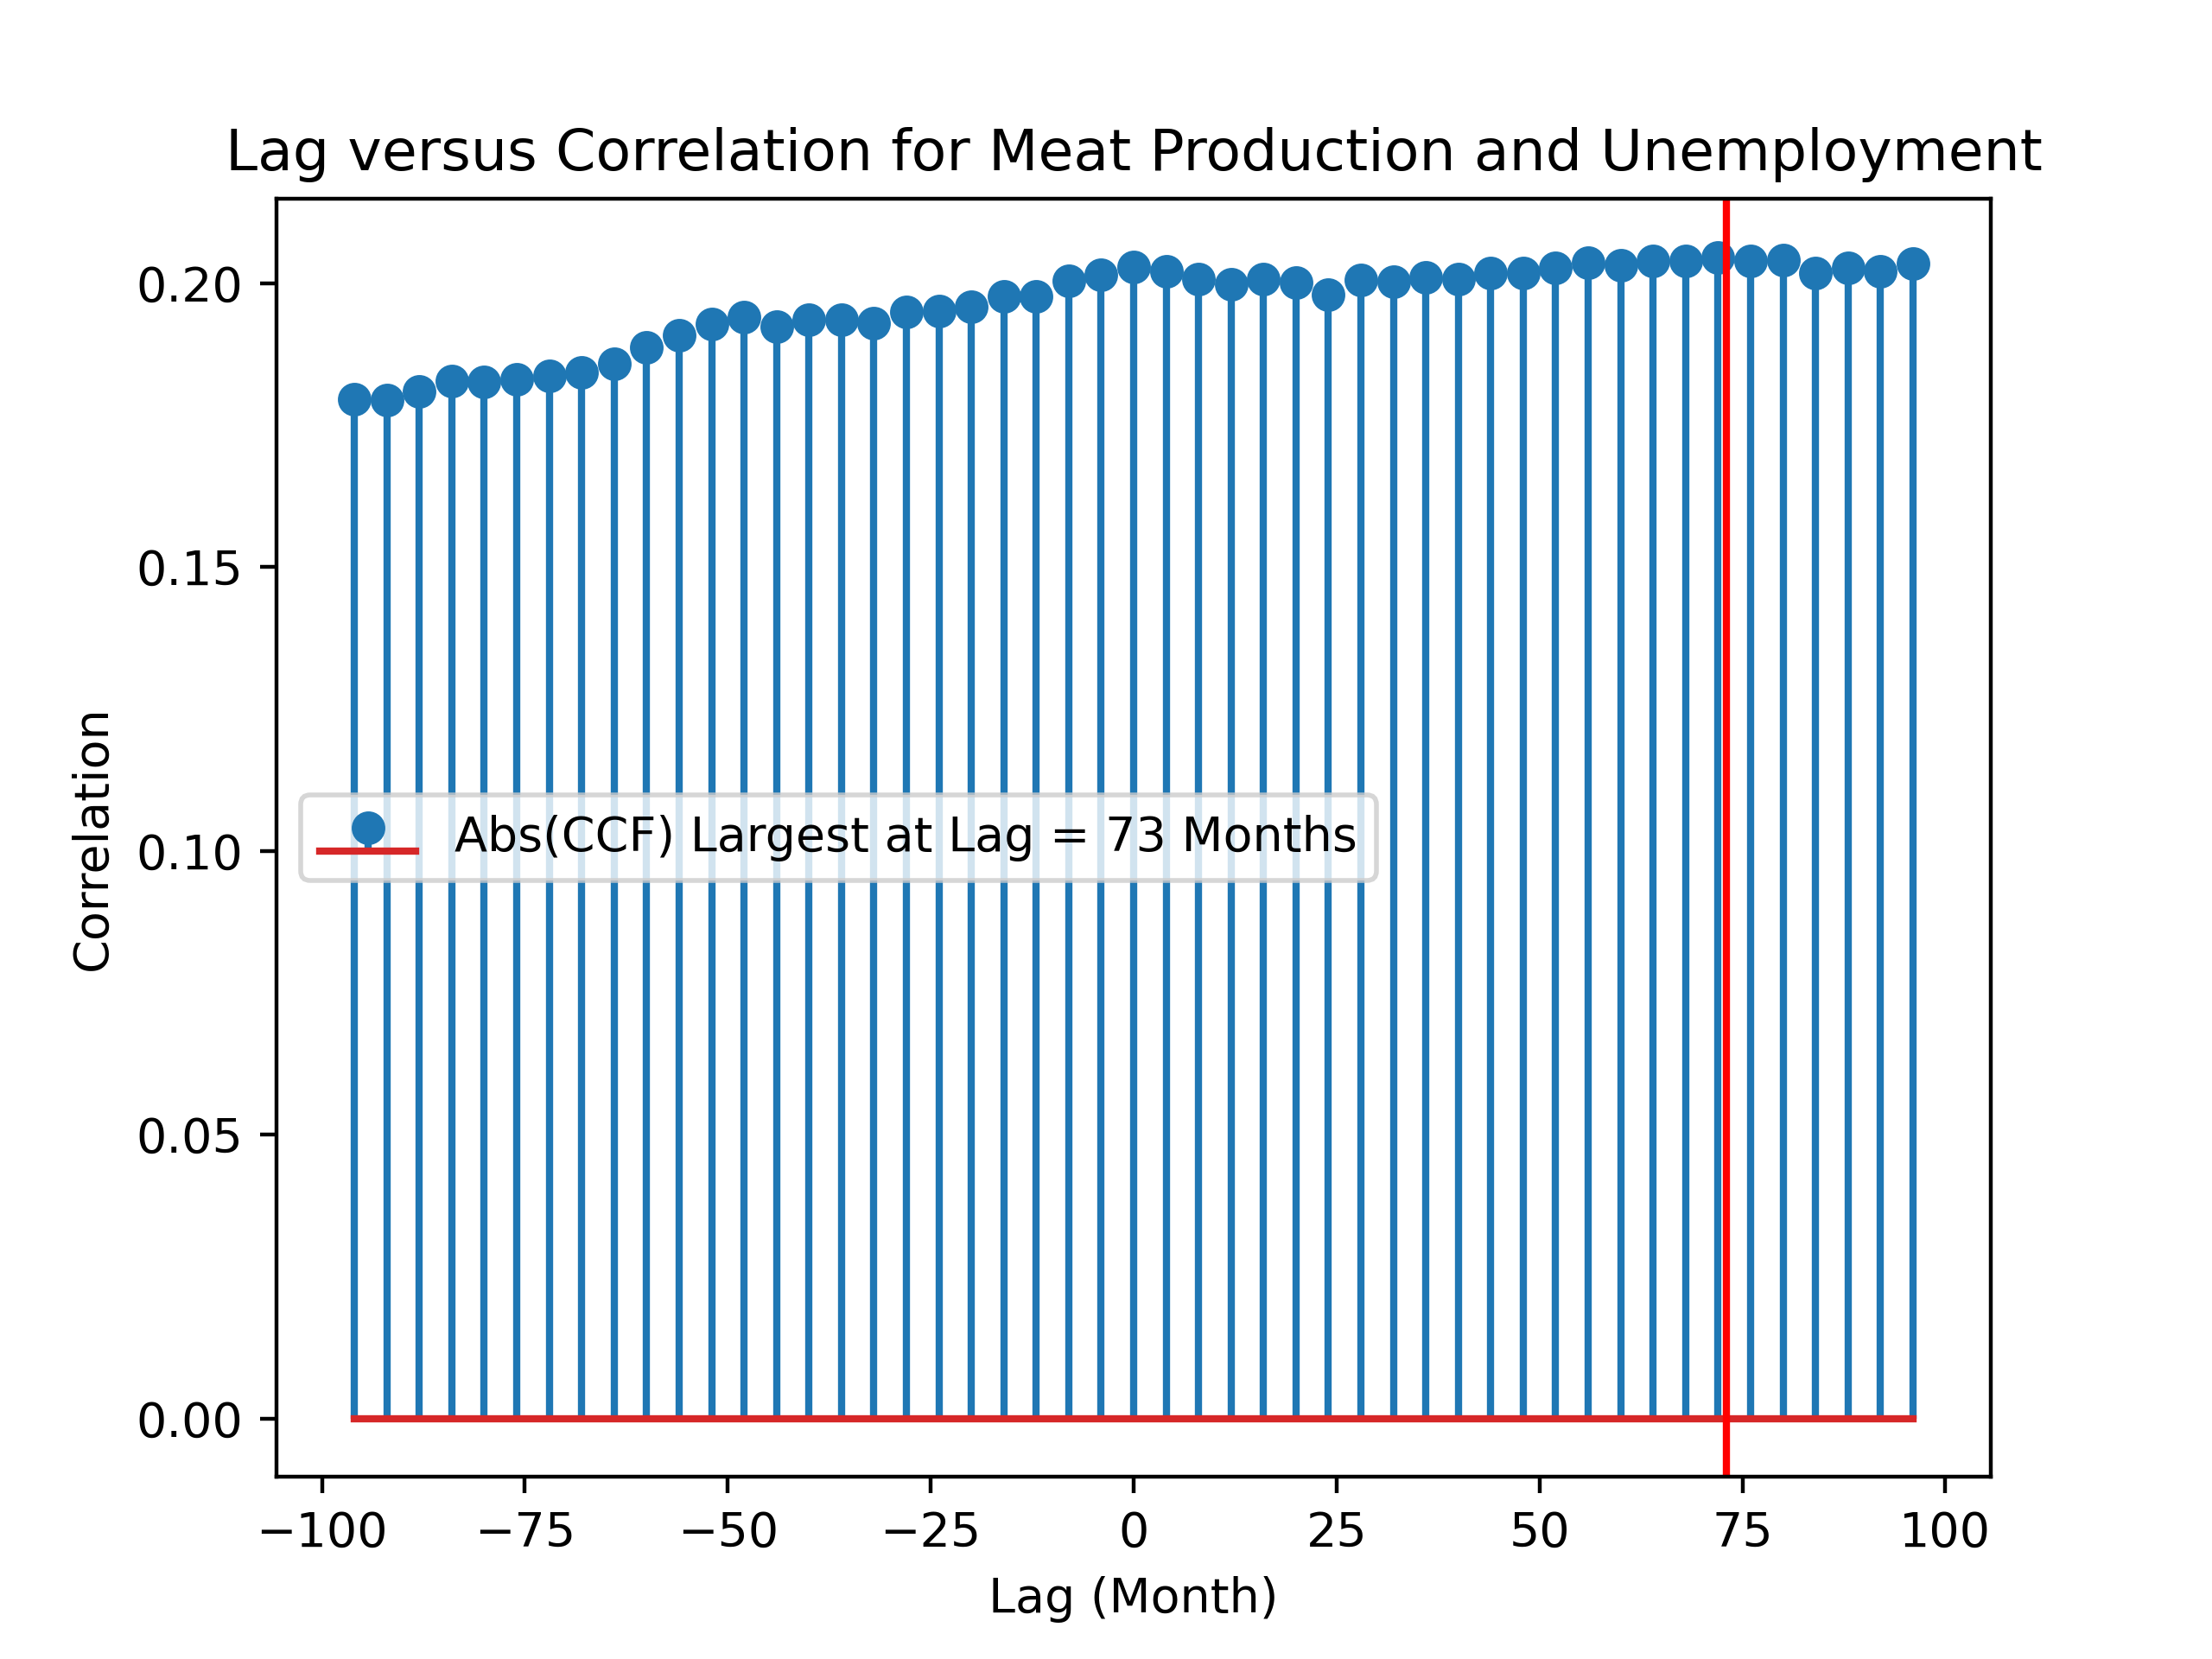
\includegraphics[width=1\linewidth]{images/Lag Correlation Coefficients - MIR.png}
        \caption{Lag Versus Correlation Using MIR}
        \label{fig:lag_mir}
    \end{minipage}
\end{figure}

Regarding our correlational study, it was clear that a non-linear, negative relationship between production and unemployment rates exists as shown in the correlation heatmap \ref{fig:7_corr_heatmap}. A $-0.51$ Kendall-Tau correlation points to meat production drawing downwards as unemployment threatens to go up, thus implying that not only can we predict unemployment from production but we can do so very well.

\begin{figure}[H]
    \centering
    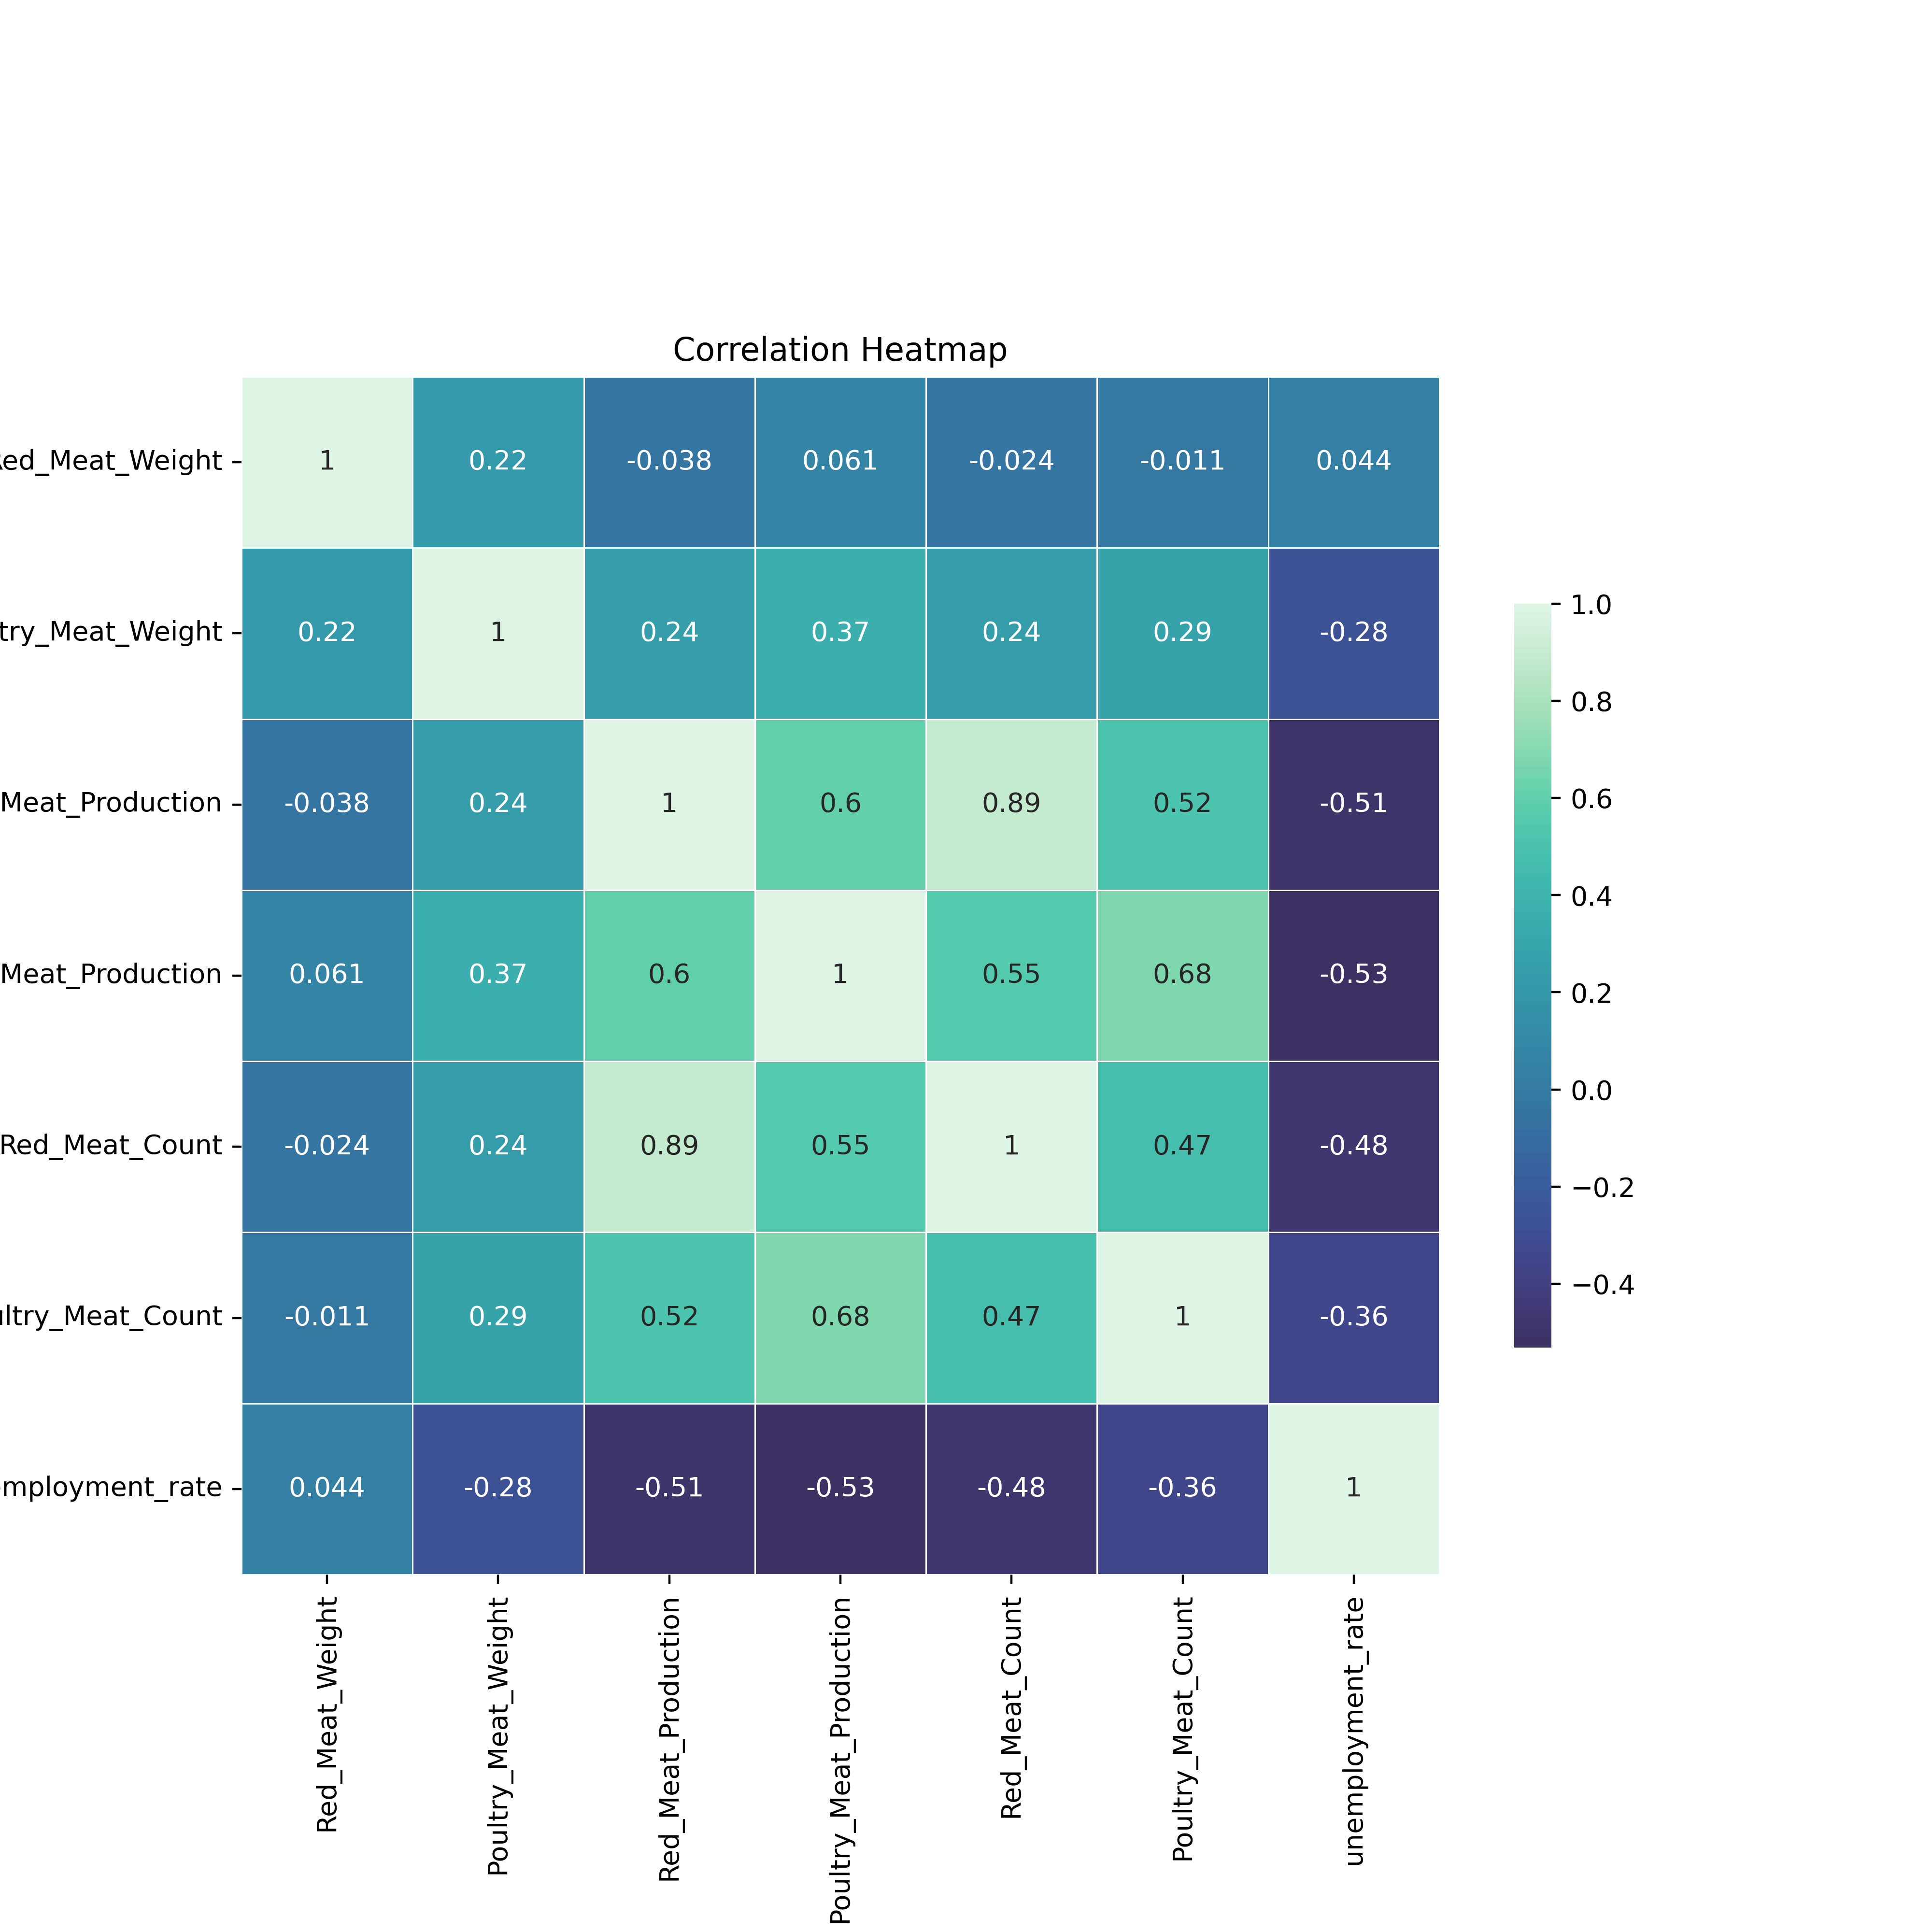
\includegraphics[width=1\linewidth]{images/Correlation Heatmap.png}
    \caption{Correlation Heatmap}
    \label{fig:7_corr_heatmap}
\end{figure}

We used the interpolated unemployment data (\ref{fig:2_monthly_unemployment}) and the monthly red meat production data as inputs for the $\mathrm{ARIMAX}(1,1,0)$ model. We chose this over the time interval where the data intersects, which is from January 2010 to December 2022.
The implementation of ARIMAX comes from the $\texttt{statsmodels}$ (version $0.14.1$) package for Python \cite{seabold2010statsmodels}. In the presence of meat data, the parameters were unable to converge. However, plotting the error (see \ref{fig:arimax-error}), we found that the mean prediction deviated at most $0.1344$ from the observed unemployment rate. 

\begin{figure}[H]
    \centering
    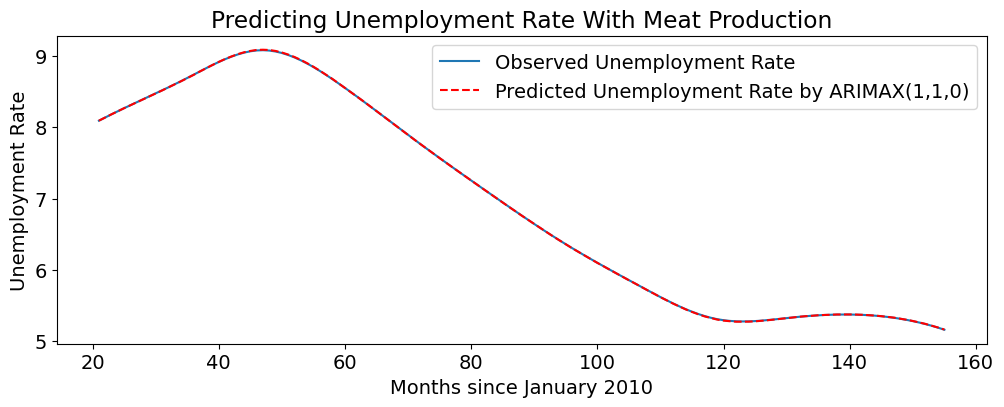
\includegraphics[width=0.6\linewidth]{images/ARIMAX Prediction.png}
    \caption{Predicted unemployment rates from $\mathrm{ARIMAX}(1,1,0)$.}
    \label{fig:arimax-predict}
\end{figure}

\begin{figure}[H]
    \centering
    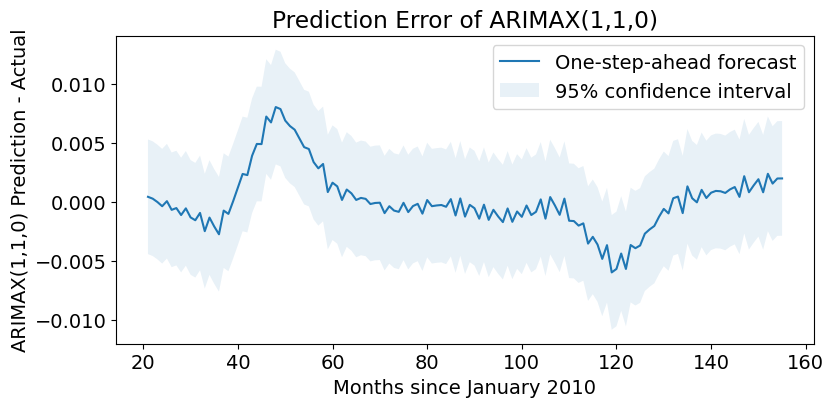
\includegraphics[width=0.6\linewidth]{images/ARIMAX Error.png}
    \caption{Error in predictions of $\mathrm{ARIMAX}(1,1,0)$.}
    \label{fig:arimax-error}
\end{figure}

We also omitted the unemployment data after January 2020 and asked the model to forecast the future unemployment rates given the meat production per month (see \ref{fig:arimax-forecast}). The model forecasted that after 30 months, in July 2022, there would be a $4.420633$ unemployment rate with a $95\%$ confidence interval of $[3.947424, 4.893841]$. 

\begin{figure}[H]
    \centering
    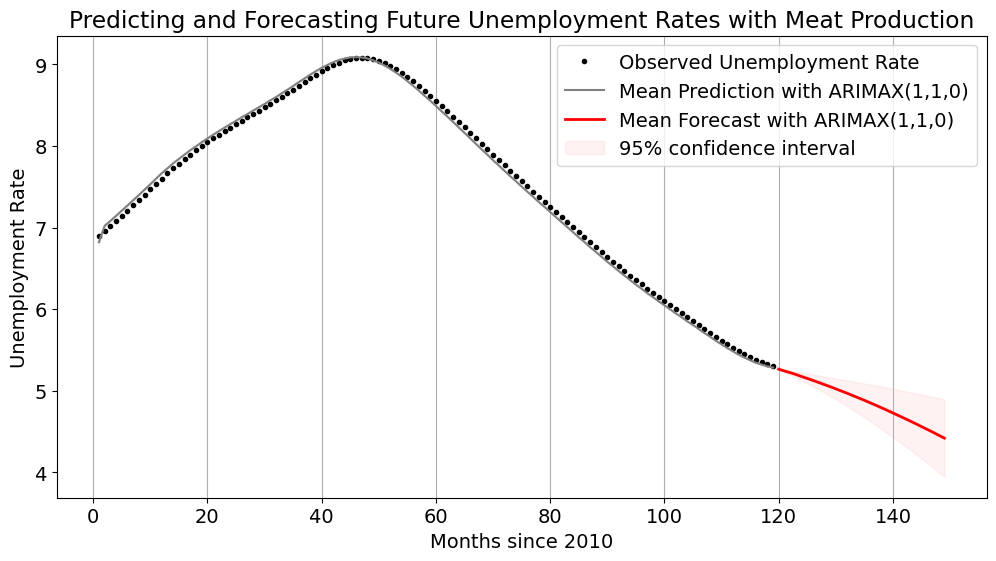
\includegraphics[width=0.6\linewidth]{images/ARIMAX Forecasting.png}
    \caption{Forecasted unemployment rates from $\mathrm{ARIMAX}(1,1,0)$.}
    \label{fig:arimax-forecast}
\end{figure}

\section{Conclusion \& Future Directions}
In this report, we considered methods such as ARIMA predicting and forecasting, lag analysis, and interpolating economic data to estimate monthly unemployment rates. Other methods may be useful when analyzing the relationship between meat production and unemployment rates, and we shall present them here as future directions to consider. For instance, although we used the cross-correlation function to calculate the correlation between the two shifted time series, we can use mutual information regression to compute this in the future. 

There is a modified version of ARIMA, \textit{SARIMA}, that accounts for seasonal changes that we encountered with our lag analysis. In the presence of more granular meat and unemployment rate data, we may have had parameters sufficiently converge for the model. We could have also experimented with other hyper-parameters (i.e. the $p,d,q$ in $\mathrm{ARIMA}(p,d,q)$).

Another possible direction to consider is to use neural networks to enhance the prediction of future meat production and unemployment rates. In particular, we could use LSTM (Long Short-Term Memory) models, which are well-suited for time-series forecasting because they can effectively learn long-term dependencies in sequential data. By training on historical data, we can use LSTM models over traditional auto-regressive ones to develop more robust predictive models of meat production and unemployment rates, potentially leading to better planning and decision-making in the meat production industry. This, of course, is conditioned on us obtaining larger quantities of data since the complex nature of neural network loss functions means instability issues can arise with smaller datasets.

Similarly, we can leverage decision-tree or neural-based architectures for extracting the relationships between the shortlisted feature-set. Although correlational analysis provides information regarding such relationships, the intense non-linearity of certain datasets can challenge such measures. With the use of model-agnostic interpreters, namely SHAP (SHapley Additive exPlanations) or RFE (Recursive Feature Elimination), we can gauge feature importance and re-structure our approach towards modeling and further analysis based on the findings; i.e., we can dive deeper into the features that matter more.

\clearpage
\bibliographystyle{plain} 
\bibliography{refs}

\end{document}
